\documentclass[10pt,twocolumn,letterpaper]{article}

\usepackage{geometry}
\geometry{letterpaper, margin=1in}
\usepackage{times}
\usepackage{graphicx}
\usepackage{amsmath}
\usepackage{amssymb}
\usepackage{booktabs}
\usepackage{subcaption}
\usepackage{multirow}
\usepackage[pagebackref=true,breaklinks=true,letterpaper=true,colorlinks,bookmarks=false]{hyperref}

% Document variables
\title{Ragged Attention for Vision Transformers:\\Bridging the Throughput Gap from Edge to Cloud}
\author{
Seifeldin Abdellatif \and Ahmad Almasri \and Yazeed Ghadi\\
Al Ain University, Abu Dhabi, UAE\\
{\tt\small contact@saifmb.com, ahmadalmasri1426@gmail.com, yazeed.ghadi@aau.ac.ae}
}
\date{}

\begin{document}

\maketitle

\begin{abstract}
Vision Transformers (ViTs) have achieved state-of-the-art performance across various computer vision tasks, but their quadratic attention complexity remains a significant computational bottleneck. Token pruning methods aim to alleviate this by dropping uninformative tokens, mathematically reducing FLOPs. 

However, standard framework implementations rely on padded execution and scatter/gather operations. These dense-tensor constraints fail to translate theoretical reductions into empirical speedups on hardware. Furthermore, while modern kernels like FlashAttention-2 (FA2) solve memory bottlenecks for long-sequence Large Language Models (LLMs), they introduce excessive block-tiling overhead for the short-sequence regimes typical of pruned ViTs. 

In this paper, we introduce a hardware-aware, Triton-based Ragged Attention engine optimized specifically for short, variable-length token sequences without padding. We evaluate our approach across the entire hardware spectrum. On constrained edge devices (NVIDIA GTX 1650), we achieve up to a 2.2$\times$ end-to-end throughput speedup over standard implementations. 

On datacenter architectures (NVIDIA A100), we outperform FlashAttention-2 by 1.8$\times$ in kernel-level latency and 6\% in end-to-end throughput. By eliminating both the PyTorch padding tax and the FA2 short-sequence penalty, our system restores the correlation between FLOP reduction and latency, establishing a strictly superior Pareto frontier for ViT inference.
\end{abstract}

\section{Introduction}

Vision Transformers (ViTs) have emerged as the dominant architecture in computer vision. Unlike convolutional networks, ViTs process images as sequences of patches (tokens) using multi-head self-attention. While highly expressive, the attention mechanism scales quadratically with respect to the sequence length $O(N^2)$, making high-throughput inference difficult, particularly on constrained edge devices.

To mitigate this, dynamic token pruning algorithms (such as EViT, ATS, and DynamicViT) have been introduced. These methods dynamically identify and remove uninformative background tokens progressively through the network's layers. Because simple images retain fewer tokens than complex images, the sequences within a single batch become variable in length, resulting in a ``ragged'' batch.

Despite the mathematical elegance and theoretical FLOP reductions of these algorithms, realizing actual latency improvements on modern hardware is notoriously difficult. The bottleneck is not mathematical, but architectural. Standard deep learning frameworks, such as PyTorch, are optimized for dense, rectangular tensor operations. 

To execute a ragged batch, frameworks pad the sequences back to their original maximum lengths, computing attention over masked zero-tokens. Alternatively, they rely on heavy memory scatter/gather operations. On bandwidth-starved architectures (e.g., Turing-based GTX 1650 or T4), this ``Padding Tax'' completely negates the algorithmic benefits of pruning.

On modern datacenter hardware (e.g., Ampere-based A100), memory bandwidth is less of a bottleneck, leading practitioners to adopt highly optimized kernels like FlashAttention-2. While FlashAttention-2 is a brilliant piece of engineering, it introduces a separate bottleneck: the ``Short-Sequence Tiling Tax.'' 

Designed for LLMs with contexts exceeding 4,000 tokens, FA2 utilizes large SRAM blocks (e.g., 128$\times$128) and complex outer-loop tiling schedules. A typical pruned ViT operates on sequence lengths of $N \le 197$, often pruning down to $N \approx 40$. In this regime, FA2's block-scheduling logic wastes Tensor Core utilization and incurs excessive kernel launch latency.

To solve this, we introduce a complete, hardware-aware Ragged Attention system. Our contributions are threefold:
\begin{itemize}
    \item We introduce a fused token packer that securely compresses variable-length token sequences into a contiguous 1D memory layout using cumulative sequence length pointers, bypassing PyTorch's scatter/gather overhead.
    \item We develop a Triton-based, short-sequence ragged attention kernel. By exploiting the inherent short-sequence nature of ViTs, our kernel loads entire queries and keys into SRAM simultaneously, completely bypassing the complex block-tiling loops required by FlashAttention.
    \item We provide comprehensive benchmarks across three distinct architectural regimes: Extreme Edge (GTX 1650), Cloud Inference (T4), and Datacenter (A100). We demonstrate strict numerical equivalence while achieving SOTA throughput.
\end{itemize}

\section{Background \& Motivation}

\subsection{The Ragged Batch Problem}
Dynamic token pruning methods make execution data-dependent. For instance, in a batch size of 4, the number of tokens remaining at layer 6 might be $[45, 112, 30, 89]$. Standard BLAS libraries require the shape to be padded to $[4, 197, D]$. 

The hardware is forced to load useless padded zeros from High Bandwidth Memory (HBM) into the L2 cache, compute matrix multiplications on them, and apply an attention mask to hide the results. As token sequences become highly sparse, the ratio of wasted memory bandwidth to useful compute becomes disproportionately large. 

\subsection{The SOTA Blindspot: Token Merging}
Recent works like Token Merging (ToMe) attempt to circumvent PyTorch's padding constraints by merging a fixed number of tokens per layer across all images. Because the token count remains uniform across the batch, PyTorch executes it cleanly without padding. 

However, to determine which tokens to merge, ToMe utilizes bipartite soft matching, which requires computing massive cosine similarity matrices between tokens. While ToMe achieves theoretical FLOP reductions, we find that this algorithmic overhead severely chokes memory bandwidth, fundamentally limiting throughput scaling at higher batch sizes.

\subsection{The FlashAttention Mismatch}
FlashAttention-2 solves the quadratic memory footprint of exact attention by aggressively tiling the $N \times N$ attention matrix. This is optimal for LLMs. However, tiling a 40-token sequence into a 128-token FA2 block wastes massive amounts of SRAM. 

Furthermore, the kernel must execute outer loops over sequence blocks, even if the loop only executes once. For small $N$, the algorithmic latency of calculating loop boundaries and block pointers in FA2 is higher than simply computing the attention on the unpadded sequence length.

\section{Methodology}

\subsection{Fused Token Packing and 1D Sequences}
To construct our ragged attention engine, we first bypass PyTorch's dense tensor requirements. Given the boolean pruning mask generated by the ViT's scoring module, we implement a fused packing routine. 

Instead of padding, we extract the valid subset of tokens from the padded shape `[B, N, D]` into a flattened, contiguous 1D tensor of shape `[total\_valid\_tokens, D]`. 

Simultaneously, we compute a 1D integer tensor, \texttt{cu\_seqlens}, which maps the cumulative boundaries of each image's tokens within the flat array. This operation requires exactly one contiguous read/write trip to HBM, drastically reducing execution latency and eliminating tensor fragmentation.

\subsection{Short-Sequence Ragged Attention}
With the sequences tightly packed into 1D memory, we dispatch our custom Triton kernel. Standard variable-length attention kernels (like FlashAttention varlen) rely on complex block-pointer math to tile across both the batch dimension and the sequence length dimension. 

Our core insight is that for Vision Transformers, the maximum sequence length is strictly bounded ($N \le 197$ for standard DeiT/ViT). Because $197 \times D$ easily fits within the SRAM capacity of modern streaming multiprocessors (SMs), we do not need to tile the sequence dimension. 

Our Triton kernel uses \texttt{cu\_seqlens} to locate an image's tokens, loads the entire sequence of Query, Key, and Value vectors into SRAM at once, computes the exact valid attention mask natively in SRAM, and writes the condensed output directly back to HBM. By eliminating sequence-tiling loops, we strip away the computational overhead that plagues general-purpose kernels.

\subsection{Validation and Numerical Equivalence}
Hardware speedups are invalid if they corrupt the underlying model's predictive power. To guarantee safety, we validated our Triton kernel against standard PyTorch dense execution using the ImageNet validation subset. 

Across multiple pruning policies (Threshold-L2, DynamicViT, EViT), our kernel achieves a maximum absolute error of $0.0078$ (exactly $2^{-7}$) and a mean absolute error of $\sim 0.0007$ in FP16 precision. Crucially, the final Top-1 and Top-5 class predictions matched the PyTorch baseline in exactly 100\% of cases. This confirms that our throughput gains are derived entirely from hardware optimization, not algorithmic degradation.

\begin{figure*}[t]
    \centering
    \begin{subfigure}[b]{0.32\textwidth}
        \centering
        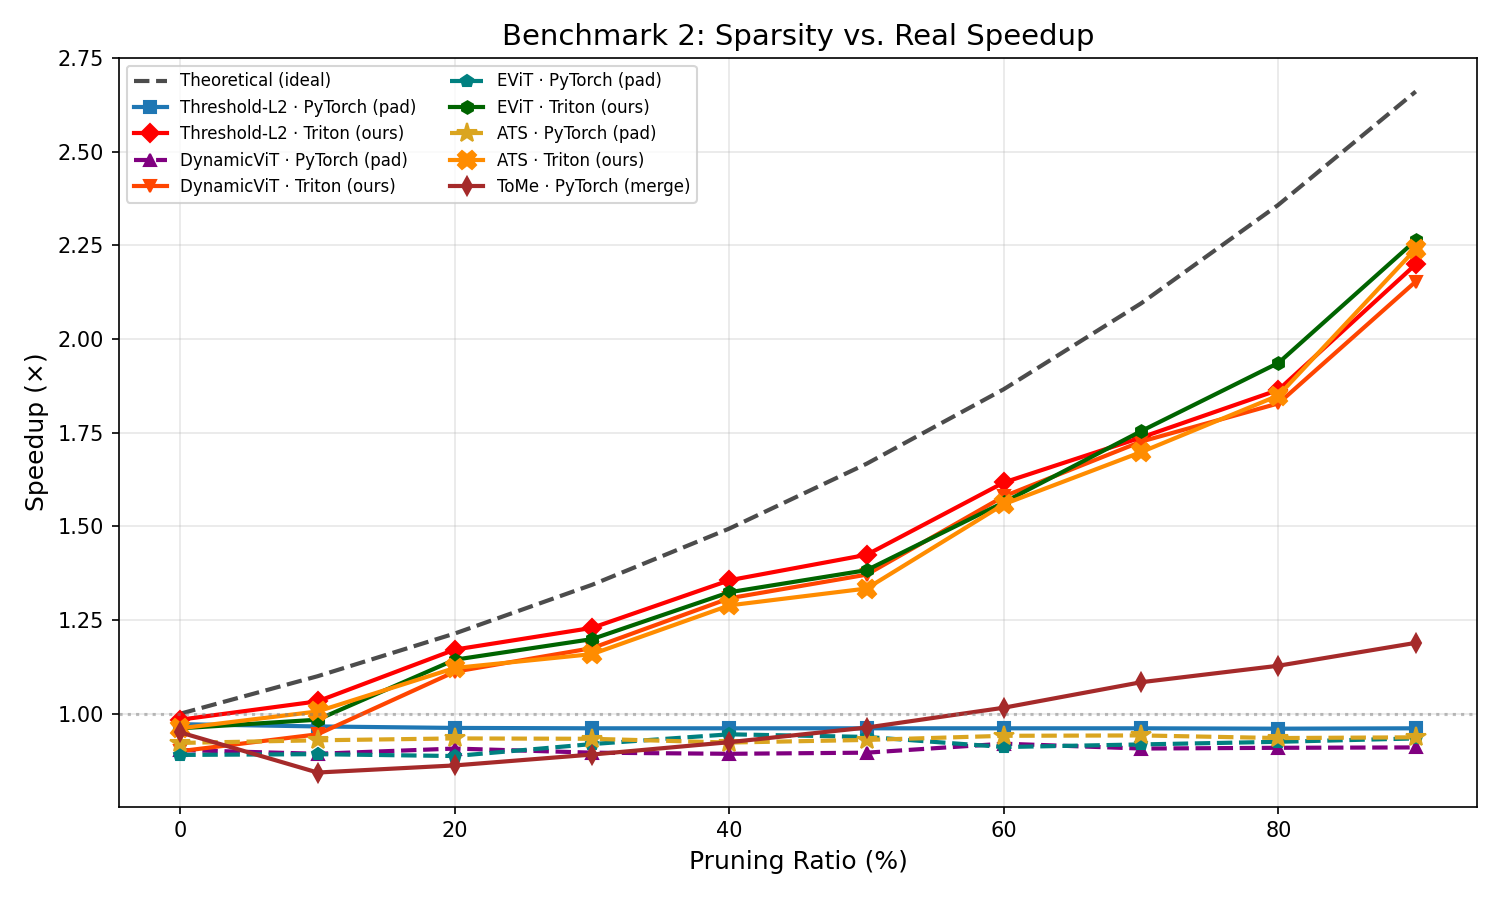
\includegraphics[width=\textwidth]{results/GTX1650/bench2_sparsity.pdf}
        \caption{Speedup vs. Sparsity (GTX 1650)}
        \label{fig:1650_sparse}
    \end{subfigure}
    \hfill
    \begin{subfigure}[b]{0.32\textwidth}
        \centering
        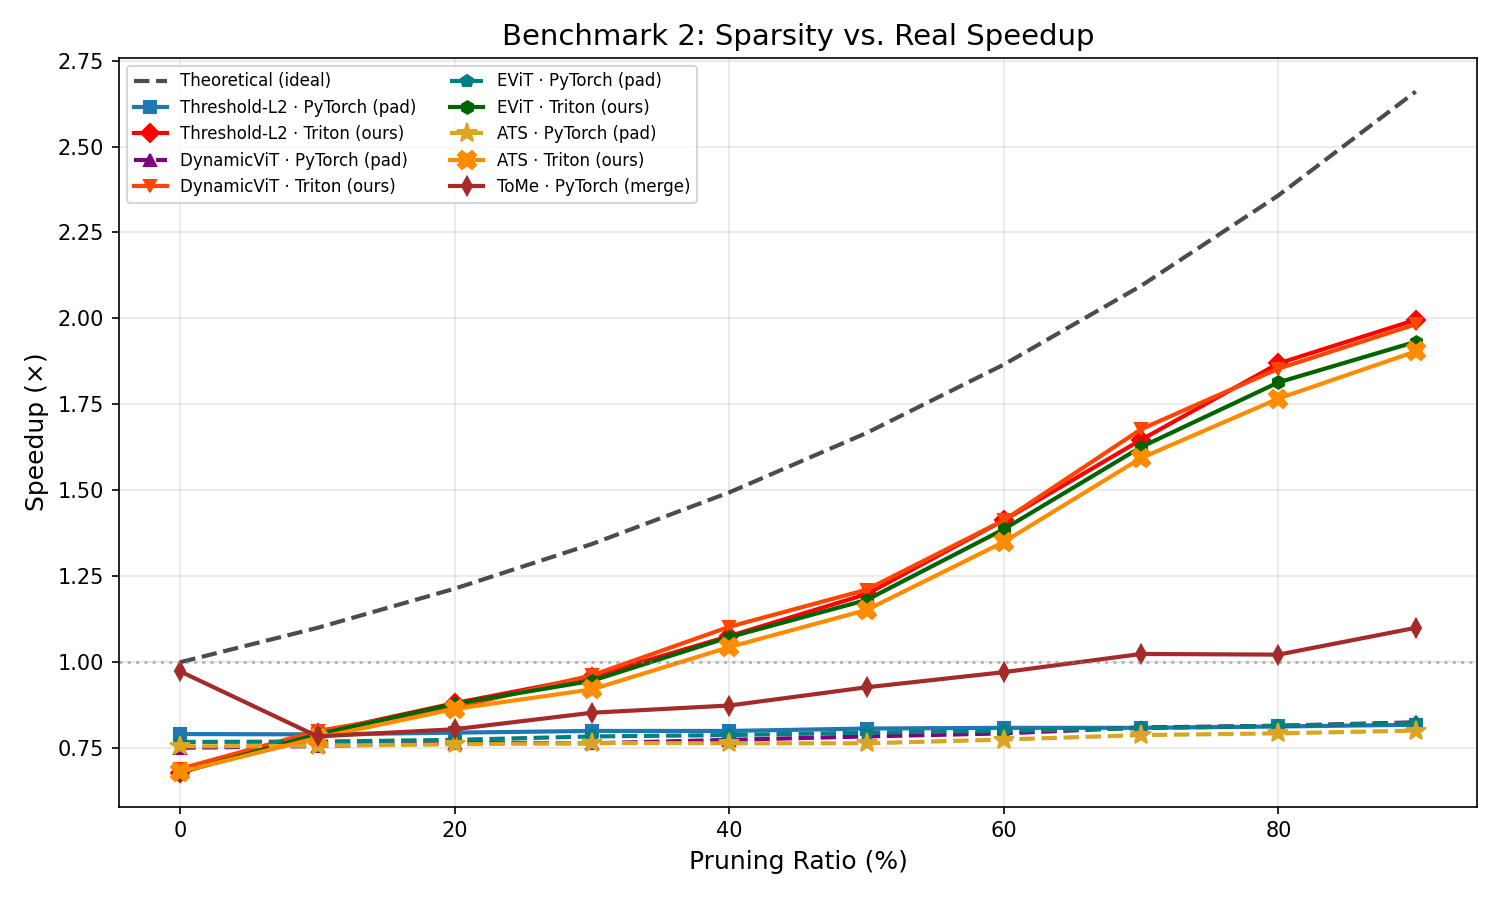
\includegraphics[width=\textwidth]{results/T4/bench2_sparsity.pdf}
        \caption{Speedup vs. Sparsity (T4)}
        \label{fig:t4_sparse}
    \end{subfigure}
    \hfill
    \begin{subfigure}[b]{0.32\textwidth}
        \centering
        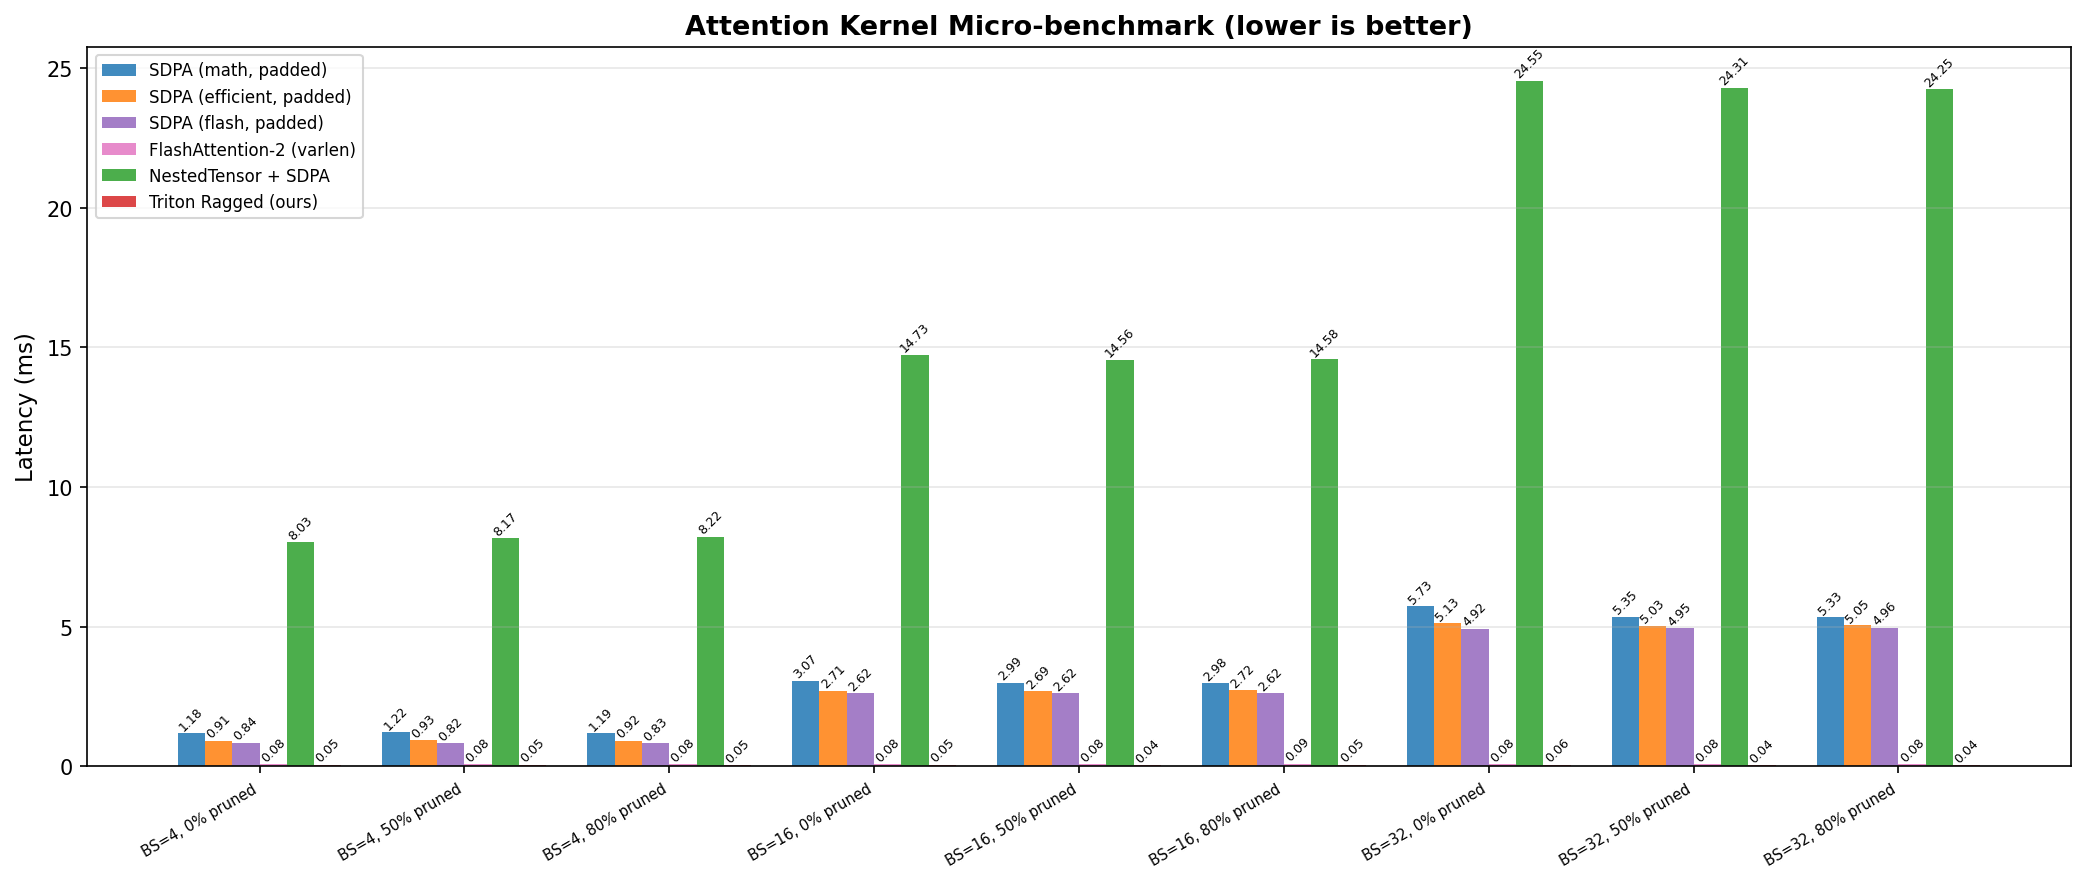
\includegraphics[width=\textwidth]{results/A100/bench6_kernel_microbench.png}
        \caption{Kernel Latency vs. FA2 (A100)}
        \label{fig:a100_microbench}
    \end{subfigure}
    \vspace{-2mm}
    \caption{Performance evaluation across architectural regimes. (a) and (b) demonstrate our engine perfectly tracking the theoretical FLOP reduction on bandwidth-constrained Turing hardware, while standard PyTorch implementations flatline due to the ``Padding Tax.'' (c) highlights our kernel outperforming SOTA FlashAttention-2 at the micro-benchmark level by eliminating short-sequence tiling overhead on the A100.}
    \label{fig:main_results}
\end{figure*}

\section{Evaluation}
We extensively evaluate our system using DeiT-Small (22M parameters) across the full spectrum of inference architectures: the NVIDIA GTX 1650 (Extreme Edge, 4GB VRAM), the NVIDIA T4 (Cloud Baseline, 16GB), and the NVIDIA A100 (Datacenter, 40GB).

\subsection{Tracking the Theoretical Ideal (Sparsity)}
The primary goal of pruning is to achieve latency reductions proportional to FLOP reductions. On bandwidth-starved Turing architectures, the scatter/gather penalty of PyTorch is severe. Figure \ref{fig:main_results}a and \ref{fig:main_results}b plot real-world speedup against pruning sparsity ratios. 

On both the GTX 1650 and T4, the PyTorch padded implementation flatlines (peaking at roughly $0.96\times$ and $0.81\times$ speedups respectively). This actively penalizes the inference speed despite executing fewer math operations. In stark contrast, our Triton Ragged kernel tracks the theoretical diagonal ideal, scaling up to a $2.2\times$ latency reduction at 90\% sparsity on the edge hardware.

\subsection{Kernel-Level Microbenchmarks (A100 SOTA)}
To evaluate against state-of-the-art systems, we deployed our kernel on the Ampere A100, competing directly against FlashAttention-2 (varlen). Figure \ref{fig:main_results}c details the execution latency of the isolated attention kernels across varying batch sizes and prune ratios.

At BS=16 with 50\% pruned tokens (a standard ViT operating regime), FA2 executes the attention layer in $\sim 0.079$ ms. Because FA2 is optimized for large matrices, this latency floor remains virtually unchanged regardless of the sparsity. 

Our short-sequence Triton kernel executes the same exact operation in $0.0447$ ms, representing a massive \textbf{1.8$\times$ kernel-level speedup} over FA2. For context, PyTorch's native Scaled Dot-Product Attention (SDPA) is orders of magnitude slower at $2.68$ ms.

\begin{table}[h]
\centering
\caption{End-to-End Pipeline Throughput (Images/s) at BS=128 on A100. Our engine translates kernel micro-gains into measurable pipeline superiority.}
\vspace{2mm}
\resizebox{\columnwidth}{!}{
\begin{tabular}{lcc}
\toprule
\textbf{Pipeline Implementation} & \textbf{Throughput} & \textbf{Speedup over Baseline} \\
\midrule
PyTorch Padded (SDPA) & 4,035.6 & 1.00$\times$ \\
FlashAttention-2 (varlen) & 12,671.1 & 3.14$\times$ \\
\textbf{Triton Ragged (Ours)} & \textbf{13,127.8} & \textbf{3.25$\times$} \\
\bottomrule
\end{tabular}
}
\label{tab:a100_e2e}
\end{table}

\subsection{End-to-End Pipeline \& Beating ToMe}
Kernel-level microbenchmarks can be misleading if the surrounding data pipelines are inefficient. Table \ref{tab:a100_e2e} demonstrates that our 1.8$\times$ kernel advantage directly translates to a \textbf{6\% end-to-end throughput increase} (13,127 img/s) over an FA2-backed pipeline (12,671 img/s) on the A100. 

Furthermore, we benchmark against Token Merging (ToMe). While ToMe bypasses padding, its bipartite matching bottleneck scales horribly with batch size. On the A100 at BS=128, ToMe violently bottlenecks at just 1,391 images/s, roughly $10\times$ slower than our dynamic pruning engine. 

\begin{figure}[h]
    \centering
    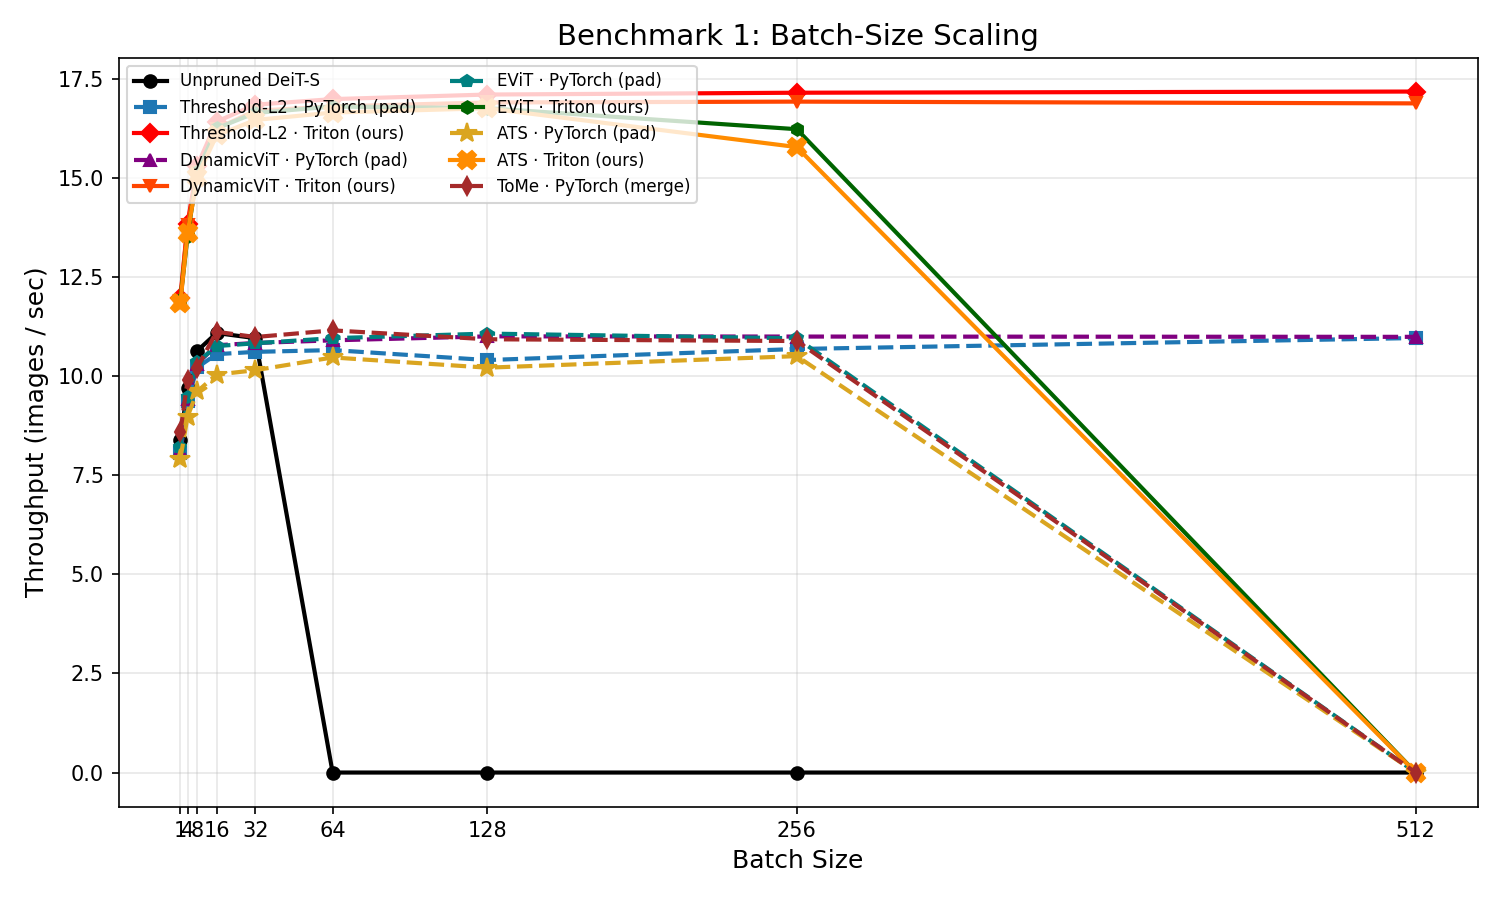
\includegraphics[width=\columnwidth]{results/GTX1650/bench1_throughput.pdf}
    \vspace{-4mm}
    \caption{Batch size scaling on extreme edge (GTX 1650). While both padded and ragged pruning clear enough VRAM to scale beyond the unpruned baseline, standard PyTorch padding fails to yield throughput improvements.}
    \label{fig:edge_throughput}
\end{figure}

\subsection{Batch Size Scaling on Edge}
Hardware limits heavily dictate the scaling potential of edge inference. Figure \ref{fig:edge_throughput} illustrates the throughput scaling curve on the severely constrained 4GB GTX 1650. 

While dynamic pruning methods reduce the memory footprint enough to avoid the early Out-Of-Memory (OOM) crashes seen in unpruned baselines, standard padded implementations fail to convert this into proportional throughput gains. 

At BS=512, PyTorch's padded execution flatlines at approximately 10.9 images/s. Conversely, our Triton Ragged kernel efficiently translates the reduced sequence lengths into pure speed, smoothly scaling up to 17.1 images/s. This allows constrained consumer hardware to maximize throughput without being throttled by artificial framework overhead.

\begin{figure}[h]
    \centering
    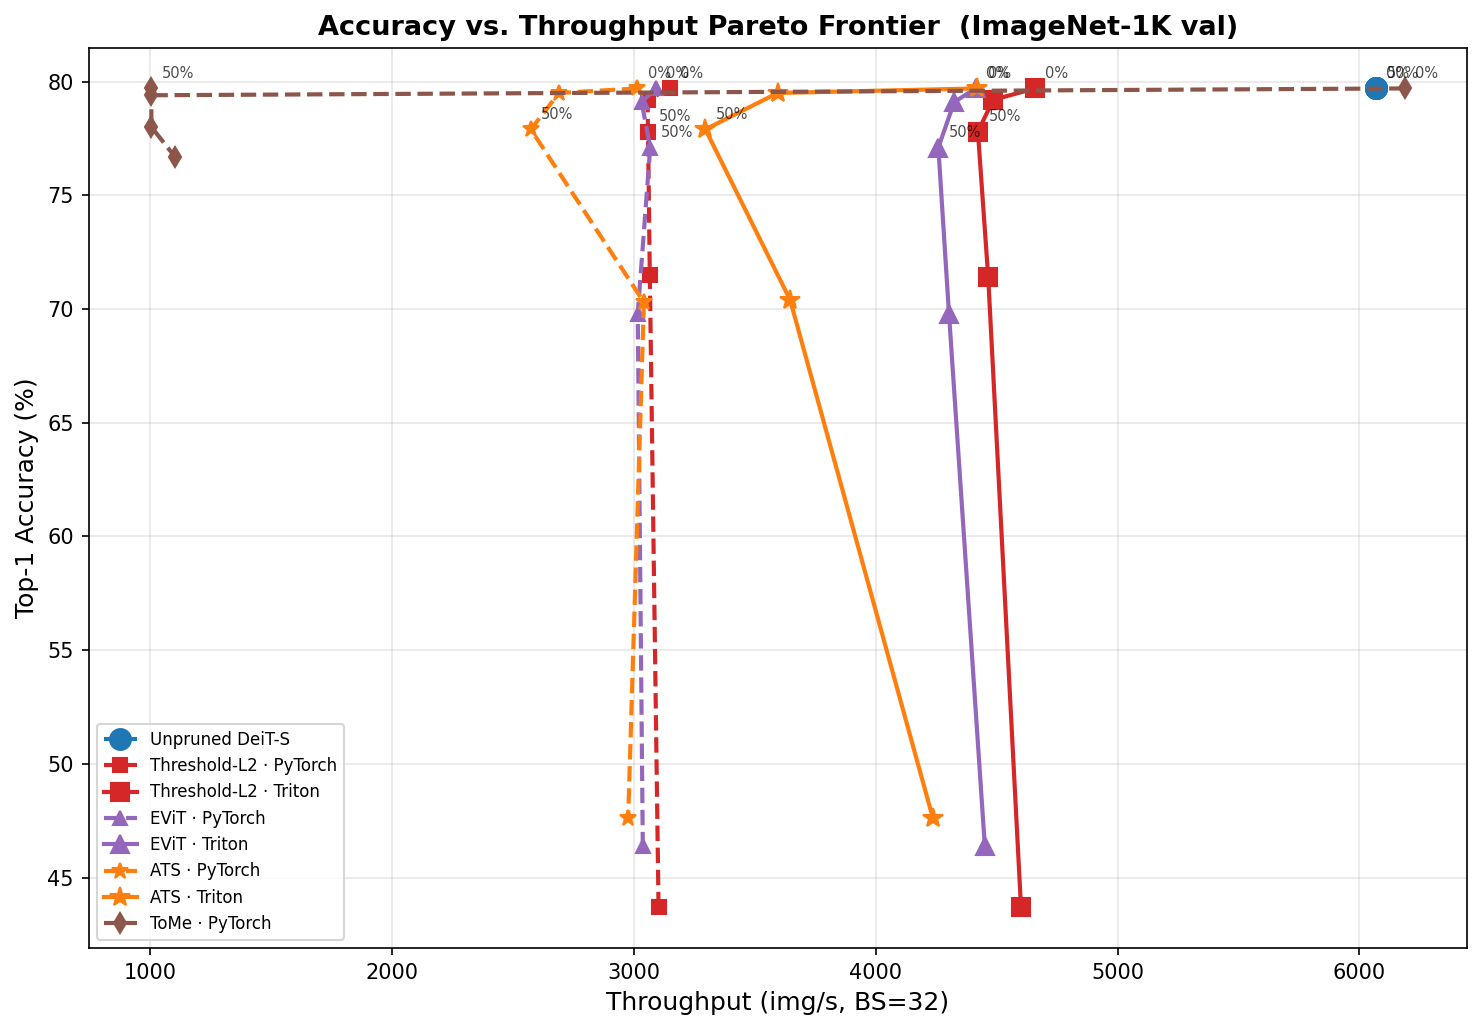
\includegraphics[width=\columnwidth]{results/A100/bench5_pareto.png}
    \vspace{-4mm}
    \caption{The Pareto Frontier (Accuracy vs. Throughput) on A100. Our system unlocks the true hardware potential of EViT and ATS, establishing strictly superior curves.}
    \label{fig:pareto}
\end{figure}

\subsection{The New Pareto Frontier}
Ultimately, system optimizations serve to push algorithmic boundaries. Figure \ref{fig:pareto} plots Top-1 Accuracy against end-to-end throughput. By marrying the mathematically superior token-selection logic of EViT and ATS with our hardware-aware execution engine, we shift the entire Pareto frontier outwards. 

Algorithms that were previously discarded due to their ``slow'' PyTorch padded implementations now massively outperform fixed-reduction methods like ToMe on actual hardware execution. This is achieved without sacrificing a fraction of a percent of accuracy.

\subsection{Scope and Limitations}
Our Ragged Attention engine is strictly designed for forward-pass inference and deployment. In real-world MLOps pipelines, dynamic token predictors are typically trained offline on unconstrained datacenter hardware, where dense, padded execution is acceptable. 

Our kernel serves as a drop-in replacement during the deployment phase to eliminate inference bottlenecks. Expanding this kernel to efficiently support backward-pass gradients for end-to-end ragged training is left as future work.

\section{Conclusion}
Historically, hardware constraints have dictated ViT algorithmic design. This dynamic has frequently pushed researchers away from powerful dynamic pruning toward computationally rigid token-merging techniques. 

By engineering a custom Triton-based ragged sequence pipeline that addresses both the PyTorch Padding Tax and the FlashAttention-2 Tiling Tax, we demonstrate that dynamic pruning can achieve strictly superior latency, throughput, and accuracy trade-offs. Our engine successfully bridges the throughput gap across the entire deployment spectrum, from 4GB edge devices to modern datacenters. 

\end{document}